\chapter{Modelling the \con{Person} Class}
\label{chap:person}
\taskstart 

In this Chapter you will:
\begin{enumerate}
%\item Create a basic ontology for the \fhkb;
\item Create a \con{Person} class;
\item Describe \con{Sex} classes;
\item Define \con{Man} and \con{Woman};
\item Ask which of the people in the \fhkb has a father.
\item Add domains and ranges to the properties in the \fhkb.
\item Make the \fhkb inconsistent.
\item  Add some more defined classes about people and see some equivalence  inferred between classes.
\end{enumerate}
These simple classes will form the structure for the whole \fhkb.


\section{The Class of Person}

For the \fhkb, we start by thinking about the objects involved
\begin{enumerate}
\item The people in a family -- Robert, Richard, David, Margaret, William, Iris, Charles, Violet, Eileen, John and Peter;
\item The sex of each of those people;
\item The marriages in which they participated;
\item The locations of their births;
\item And many more\ldots
\end{enumerate}

There is a class of \con{Person} that we will use to represent all these people objects.

\steps{Create the \con{Person} class}{
\item Create a class called \con{DomainEntity};
\item Create a subclass of \con{DomainEntity} called \con{Person}.
}
%\taskcont
\noindent We use \con{DomainEntity} as a house-keeping measure. All of our ontology goes underneath this class. We can put other classes `outside' the ontology, as siblings of \con{DomainEntity}, such as `probe' classes we wish to use to test our ontology.

The main thing to remember about the \con{Person} class is that we are using it to represent all `people' individuals. When we make statements about the \con{Person} class, we are making statements about all `people' individuals.

What do we know about people? All members of the \con{Person} class have:
\begin{itemize}
\item Sex -- they are either male or female;
\item Everyone has a birth year;
\item Everyone has a mother and a father.
\end{itemize}
There's a lot more we know about people, but we will not mention it here.


\section{Describing Sex in the \fhkb}
\label{sec:sex}

Each and every person object has a sex. In the \fhkb we will take a simple view on sex -- a person is either male or female, with no intersex or administrative sex and so on. Each person only has one sex.

We have two straight-forward options for modelling sex:
\begin{enumerate}
\item Each person object has their own sex object, which is either male or female. Thus Robert's maleness is different from David's maleness.
\item There is only one Maleness object and one Femaleness object and each person object has a relationship to either one of these sex objects, but not both.
\end{enumerate}
\noindent We will take the approach of having a class of Maleness objects and a class of Femaleness objects. These are qualities or attributes of self-standing objects such as a person. These two classes are disjoint, and each is a subclass of a class called \con{Sex}. The disjointness means that any one instance of \con{Sex} cannot be both an instance of \con{Maleness} and an instance of \con{Femaleness} at once. We also want to put in a covering axiom on the class \con{Sex}, which means that any instance of \con{Sex} must be either \con{Maleness} or \con{Femaleness}; there is no other kind of \con{Sex}.\herebedragons 

Again, notice that we have been thinking at the level of objects. We do the same when thinking about \person and their \sex. Each and every person is related to an instance of \con{Sex}. Each \person holds one relationship to a \con{Sex} object. To do this we create an object property called \con{hasSex}. We make this property functional, which means that any object can hold that property to only one distinct filler object. 

We make the domain of \con{hasSex} to be \person and the range to be \con{Sex}. The domain of  \person means that any object holding that property will be inferred to be a member of the class \person. Putting the range of \con{Sex} on the \con{hasSex} property means that any object at the right-hand end of the \con{hasSex} property  will be inferred to be of the class \con{Sex}. Again, think at the level of individuals or objects.

We now put a restriction on the \person class to state that each and every instance of the class \person holds a \con{hasSex} property with an instance of the \con{Sex} class. It has an existential operator `some' in the axiom, but the functional characteristic means that each \person object will  hold only one \con{hasSex} property to a distinct instance of a \con{Sex} object\footnote{An individual could hold two \con{hasSex} properties, as long as the sex objects at the right-hand end of the property are not different.}.

\steps{Modelling sex}{
\item Create a class called \con{Sex};
\item Make it a subclass of \con{DomainEntity};
\item Make \con{Person} and \con{Sex} disjoint;
\item Create two subclasses of \con{Sex}, \male and \female;
\item Make \male and \female disjoint;
\item Put a covering axiom on \sex such that it is equivalent to \con{Maleness or Femaleness}.
\item Create an object property, \con{hasSex}, with the domain \person, the range \con{Sex} and give it the characteristic of `Functional';
\item Add a restriction \con{hasSex some Sex} to the class \person.
}
%\taskcont

The \con{hasSex} property looks like: \\\\
\owlcode{
ObjectProperty: hasSex

    Characteristics: 
        Functional
    
    Domain: 
        Person
    
    Range: 
        Sex
}

The \person class looks like: \\\\
\owlcode{
Class: Person
    
SubClassOf:  DomainEntity,(hasSex some Sex)
    
DisjointWith:  Sex
}

\section{Defining Man and Woman}

We now have some of the foundations  for the \fhkb. We have the concept of \person, but we also need to have the concepts of \man and \woman. Now we have \person, together with \male and \female, we have the necessary components to define \man and \woman. These two classes can be defined as:
Any \person object that has a male sex can be recognised to be a man; any \person object that has a female sex can be recognised as a member of the class woman. Again, think about what conditions are \emph{sufficient} for an object to be \emph{recognised} to be a member of a class; this is how we create defined classes through the use of OWL equivalence axioms.

To make the \man and \woman classes do the following:
\steps{Describe men and women}{
\item Create a class \man;
\item Make it equivalent to a \con{Person that hasSex some} \male;
\item Do the same, but with \female, to create the \woman class;
\item A covering axiom can be put on the \person class to indicate that man and woman are the only kinds of person that can exist. (This is not strictly true due  to the way \con{Sex} has been described.)
\item Run the reasoner and take a look.
}

 \noindent Having run the reasoner, the \man and \woman classes should appear underneath \person \footnote{Actually in \protege, this might happen without the need to run the reasoner.}.

The \man and \woman classes will be important for use as domain and range constraints on many of the properties used in the \fhkb. To achieve our aim of maximising inference, we should be able to infer that individuals are members of \man, \woman or \person by the properties held by an object. We should not have to state the type of an individual in the \fhkb.
 
The classes for \man and \woman should look like:\\\\
\owlcode{
Class: Man
    
    EquivalentTo: 
        Person
         and (hasSex some Maleness)
\\\\
Class: Woman

    EquivalentTo: 
        Person
         and (hasSex some Femaleness)
}

%\begin{figure}
%\centering
%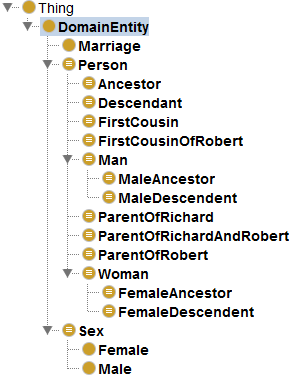
\includegraphics[width=.75\textwidth]{figures/class_hierarchy}
%\comment{WRONG TEXT, this is a Snapshot of an ADVANCED version of the class hierarchy!}
%\caption{An OWLviz picture of the \fhkb TBox as it now stands}
%\label{fig:stage1}
%\end{figure}

\section{Describing Parentage in the \fhkb}
 
To finish off the foundations of the \fhkb we need to describe a person object's parentage. We know that each and every person has one mother and each and every person has one father. Here we are talking about biological mothers and fathers. The complexities of adoption and step parents are outside the  scope of this \fhkb tutorial.

\steps{Describing Parentage}{
\item Add the domain \person and the range \woman to the property \con{hasMother}. 
\item Do the same for the property \con{hasFather}, but give it the range \man;
\item Give the property \con{hasParent} domain and range of \person;
\item Run the reasoner.
}
\noindent The (inferred) property hierarchy in the \fhkb should look like that shown in Figure~\ref{fig:phparentage}. Notice that we have asserted the sub-property axioms on one side of the property hierarchy. Having done so, the reasoner uses those axioms, together with the inverses, to work out the property hierarchy for the `other side'.

We make \con{hasMother} functional, as any one person object can hold only one \con{hasMother} property to a distinct \woman object. The range of \con{hasMother} is \woman, as a mother has to be a woman. The \person object holding the \con{hasMother} property can be either a man or a woman, so we have the domain constraint as \person; this means any object holding a \con{hasMother} property will be inferred to be a \person. Similarly, any object at the right-hand end of a \con{hasMother} property will be inferred to be a \woman, which is the result we need. The same reasoning goes for \con{hasFather} and \con{hasParent}, with the sex constraints on the latter being only \person. The inverses of the two functional sub-properties of \con{hasParent} are not themselves functional. After all, a \woman can be the mother of many \person objects, but each \person object can   have only one mother.

\begin{figure}
\begin{center}
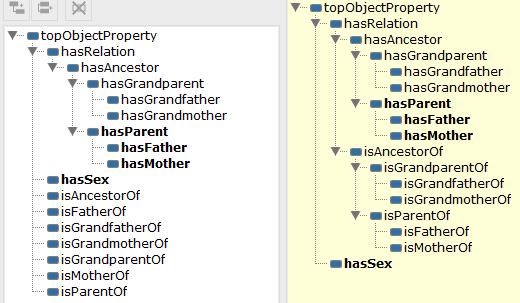
\includegraphics[width=\figwidth]{figures/new/prophierparentage}
\caption{The property hierarchy with the \con{hasSex} and the parentage properties}\label{fig:phparentage}
\end{center}
\end{figure}

\steps{Restrict \person class}{
\item As each and every person has a mother and each and every person has a father, place restrictions on the \person class as shown below.
}

\owlcode{
Class: Person
    
    SubClassOf: 
        DomainEntity,
         (hasFather some Man),
         (hasMother some Woman),
         (hasSex some Sex)
    
    DisjointWith: 
        Sex
}

\begin{figure}
\begin{center}
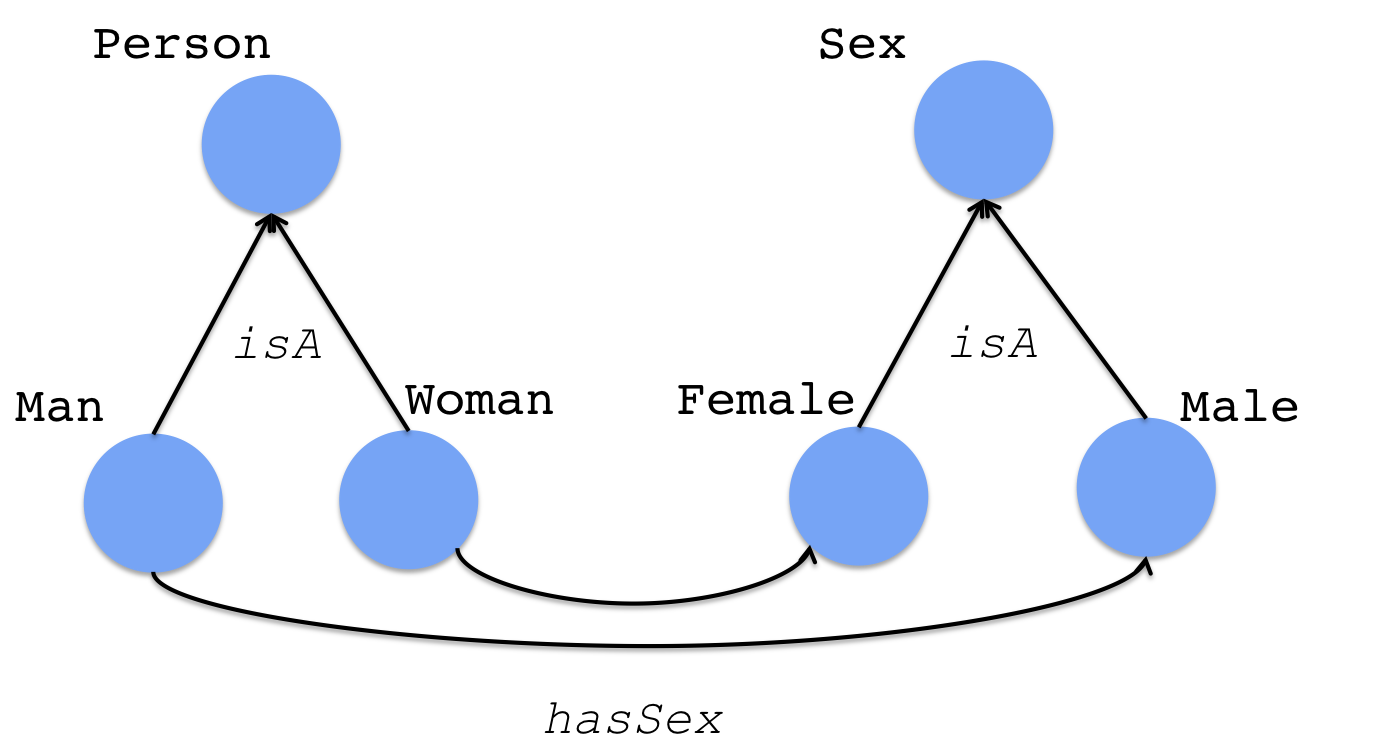
\includegraphics[width=\figwidth]{figures/sex}\caption{the core TBox for the \fhkb with the \person and \con{Sex} classes.}\label{fig:person_sex}
\end{center}
\end{figure}

\steps{DL queries for people and sex}{
\item Issue the DL queries for \person, \man and \woman; look at the answers and count the numbers in each class; which individuals have no sex and why?
\item You should find that many people have been inferred to be either \man or \woman, but some are, as we will see below, only inferred to be \person.
}

The domain and range constraints on our properties have also driven some entailments. We have not asserted that \ids is a member of \man, but the range constraint on \con{hasFather} (or the inferred domain constraint on the \con{isFatherOf} relation) has enabled this inference to be made. This goes for any individual that is the right-hand-side (either inferred or asserted) of either \con{hasFather} or \con{hasMother} (where the range is that of \woman). For \rds, however, he is only the left-hand-side of an \con{hasFather} or an \con{hasMother} property, so we've only entailed that this individual is a member of \person.

% 

%\section{Asserting an Individual's Type}
%Individuals are members of classes. We can either state to which class an individual belongs, infer to which class it belongs because of what we have said about that or another individual, or we can rely on both. Sometimes, of course, we can say or infer things about an individual that means our ontology becomes inconsistent (and we will make this happen at some point).
%
%First we need some individuals, so do the following in a new file for the individuals in the \fhkb:
%\steps{Create individuals}{
%\item Create a new ontology called \texttt{fhkb-a.owl};
%\item Create the following individuals: 
%\begin{itemize}
%\item Robert David Bright (1965;
%\item David Bright (1934;
%\item Richard John Bright (1962;
%\item Margaret Grace Rever (1934;
%\end{itemize} 
%For each individual, create a IRI fragment with the given names followed by family name, followed by birth year, each separated by underscores. 
%
%
%%Save these `bare' individuals in files \texttt{fhkb-a1} and \texttt{fhkb-a2}.
%\item For each of the individuals in file \texttt{fhkb-a1}, assert the type of each individual to be either \man or \woman, as described in the OWL below.
%\item In the file \texttt{fhkb-a2}, assert sex types about each person individual using the \con{hasSex} property. An example of such an assertion can be seen below. 
%}
%
%\owlcode{
%Individual: grant\_plinth
%	
%	Annotations:
%		label "Grant Plinth"
%
%	types:
%		Man
%
%Individual: grant\_plinth
%	
%	Annotations:
%		label "Grant Plinth"
%
%	types:
%		hasSex some Maleness
%}
%
%These are ways of asserting the \textbf{type} of an individual. In the first example above we just give the type of the individual `Grant Plinth' as Man -- the class we defined in Chapter~\ref{chap:person} as `A person with sex male'. In the second example, we are not using the \man class as a type, but we are essentially doing the same thing. By giving the type of `Grant Plinth' as \con{hasSex some Maleness}, we are making him a member of the anonymous class of those entities \con{hasSex some Sex}. We can write class expressions of an arbitrary complexity in the type of an individual. Note that the domain of \con{hasSex} is \person, so we will infer any individual holding one of those \con{hasSex} properties  to be a member of the \person class. So, these two ways of asserting sex are really just the same. Note also that  we are not naming individual sex instances, we are just relating this individual to some anonymous sex instance. As \con{hasSex} is functional, this individual is related to only one distinct sex instance.
%
%We can now use each of these ways of modelling sex of individuals to show off some inferences made by the reasoners.
%
%\steps{Run the reasoner}{
%\item Run the reasoner on file \texttt{fhkb-a1}.
%\item Issue a DL query of \man and then \woman (make sure that you are checking the correct boxes in the DL Query tab if you are using \protege);
%\item Ask the DL query \con{hasSex some Maleness} and see what results are returned.
%\item Ask the DL query \con{hasFather some Man} and see what results are returned.
%\item Load in the file \texttt{fhkb-a2} and repeat the procedure, recording your results.
%}
%
%For both the \texttt{fhkb-a1} and the \texttt{fhkb-a2}, the following results should have been seen:
%\begin{itemize}
%\item For \man or \con{hasSex some Maleness}: 
%\begin{itemize}
%\item \con{Robert\_David\_Bright\_1965}
%\item \con{David\_Bright\_1934}
%\item \con{Richard\_John\_Bright\_1962}
%\end{itemize} 
%\item For \woman or \con{hasSex some Femaleness}: \con{Margaret\_Grace\_Rever\_1934}
%\item For \con{hasFather some Man} all four family members are returned.
%\end{itemize}
\section{Who has a father?}

In our description of the \person class we have said that each and every instance of the class \person has a father (the same goes for mothers). So, when we ask the query `which individuals have a father', we get all the instances of \person back, even though we have said nothing about the specific parentage of each \person. We do not know who their mothers and fathers are, but we know that they have one of each. We know all the individuals so far entered are members of the \person class;  when  asserting the type to be either \man or \woman (each of which is a subclass of \person), we infer that each is a person. When asserting the type of each individual via the \con{hasSex} property, we know each is a \person, as the domain of \con{hasSex} is the \person class. As we have also given the right-hand side of \con{hasSex} as either \male  or \female, we have given sufficient information to recognise each of these \person instances to be members of either \man or \woman.

\section{Filling in Domains and Ranges for the \fhkb Properties}

So far we have not systematically added domains and ranges to the properties in the \fhkb. As a reminder, when a property has a domain of \con{X} any object holding that property will be inferred to be a member of class \con{X}. A domain doesn't add a constraint that only members of class \con{X} hold that property; it is a strong implication of class membership. Similarly, a property holding a range implies that an object acting as right-hand-side to a property will be inferred to be of that class. We have already seen above that we can use domains and ranges to imply the sex of people within the \fhkb.

Do the following:
\steps{Domains and Ranges}{
\item Make sure the appropriate \person, \man and \woman are domains and ranges for \con{hasFather}, \con{hasMother} and \con{hasParent}.
\item Run the reasoner and look at the property hierarchy.
\item Also look at the properties \con{hasAncestor}, \con{hasGrandparent},  \con{hasUncle} and so on; look to see what domains and ranges are found. Add any domains and ranges explicitly as necessary.
}

\warning{\protege for example in its current version (November 2015) does not visualise inherited domains and ranges in the same way as it shows inferred inverse relations.}

We typically assert more domains and ranges than strictly necessary. For example, if we say that \con{hasParent} has the domain \person, this means that every object \con{x} that is connected to another object \con{y} via the \con{hasParent} relation must be a \person. Let us assume the only thing we said about \con{x} and \con{y} is that they are connected by a \con{hasMother} relation. Since this implies that \con{x} and \con{y} are also connected by a \con{hasParent} relation (\con{hasMother} is a sub-property of \con{hasParent}) we do \emph{not} have to assert that \con{hasFather} has the domain of \person; it is implied by what we know about the domain and range of \con{hasParent}. 

In order to remove as many assertions as possible, we may therefore choose to assert as much as we know starting from the top of the hierarchy, and only ever adding a domain if we want to constrain the already inferred domain even further (or range respectively). For example, in our case, we could have chosen to assert \person to be the domain of \con{hasRelation}. Since \con{hasRelation} is symmetric, it will also infer \person to be the range. We do not need to say anything for \con{hasAncestor} or \con{hasParent}, and only if we want to constrain the domain or range further (like in the case of \con{hasFather} by making the range \con{Man}) do we need to actually assert something. It is worth noting that because we have built the object property hierarchy from the bottom (\con{hasMother} etc.) we have ended up asserting more than necessary.

\section{Inconsistencies}

From the Pizza Tutorial and other work with OWL you should have seen some \emph{unsatisfiabilities}. In \protege this is highlighted by classes going `red' and being subclasses of \con{Nothing}; that is, they can have no instances in that model.

\steps{Inconsistencies}{
\item Add the fact \irds \con{hasMother} \ids.
\item Run the classifier and see what happens.
\item Remove that fact and run the classifier again.
\item Now add the fact that \irds \con{hasMother} \iiea{}. 
\item Run the classifier and see what happens.
\item Add and remove the functional characteristic to these properties and see what happens.
}

After asserting the first fact it should be reported by the reasoner that the ontology is \emph{inconsistent}. 
This means, in lay terms, that the model you've provided in the ontology cannot accommodate the facts you've provided in the fact assertions  in your ABox---that is, there is an inconsistency between the facts and the ontology\ldots
The ontology is inconsistent because \ids is being inferred to be a \man and a \woman at the same time which is inconsistent with what we have said in the \fhkb. 
%\comment{put the justification in here and check if that is available in \protege.}

When we, however, say that \rds has two different mothers, nothing bad happens! Our domain knowledge says that the two women are different, but the reasoner does not know this as yet\ldots; Iris Ellen Archer  and Margaret Grace Rever may be the same person; we have to tell the reasoner that they are different. For the same reason the functional characteristic also has no effect until the reasoner `knows' that the individuals are different. \herebedragons We will do this in Section~\ref{sec:countchildren} and live with this	 `fault' for the moment.

%\begin{tasks}
%\item Make all the individuals different by adding a `different individuals' axiom; \comment{Add a comment; remove that axiom and reintroduce it in \ref%{sec:countchildren}}
%\item Run the reasoner and look at the results;
%\item Remove the offending axiom about \rds having Iris Elenn Archer as a mother, re-run the classifier and check the results.
%\end{tasks}
%\taskcont

\section{Adding Some Defined Classes for Ancestors and so on}
\label{sec:ancest-defined}

\steps{Adding defined classes}{
\item Add a defined class for \con{Ancestor}, \con{MaleAncestor}, \con{FemaleAncestor};
\item Add a defined class for \con{Descendant}, \con{MaleDescendant} and \con{FemaleDescendant};
\item Run the reasoner and view  the resulting hierarchy.
}
The code for the classes looks like:
\\\\
\owlcode{
Class: Ancestor
	EquivalentTo: Person
		and isAncestorOf some Person

Class: FemaleAncestor
	EquivalentTo: Woman
	and isAncestorOf some Person

Class: Descendant
	EquivalentTo: Person
		and hasAncestor some Person

Class: MaleDescendant
	EquivalentTo: Man
		and hasAncestor some Person
} 
\\\\
The TBox after reasoning can be seen in Figure~\ref{fig:equiv}. Notice that the reasoner has inferred that several of the classes are equivalent or `the same'. These are: Descendant and Person; MaleDescendant and Man, FemaleDescendant and Woman.
%\begin{itemize}
%\item Ancestor and Parent; Father and Male Ancestor; [NO! There is no Parent and Father class]
%\item 
%\end{itemize}

The reasoner has used the axioms within the ontology to infer that all the instances of \con{Person} are also instances of the class \con{Descendant} and that all the instances of \con{Woman} are also the same instances as the class \con{Female Descendant}. This is intuitively true; all people are descendants -- they all have parents that have parents etc. and thus everyone is a descendant. All women are female people that have parents etc. As usual we should think about the objects within the classes and what we know about them. This time it is useful to think about the statements we have made about \person in this Chapter -- that all instances of \person have a father and a mother; add to this the information from the property hierarchy and we know that all instances of \person have parents and ancestors. We have repeated all of this in our new defined classes for \con{Ancestor} and \con{Descendant} and the reasoner has highlighted this information.

\begin{figure}
\begin{center}
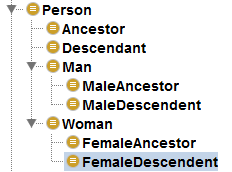
\includegraphics[width=\figwidth]{figures/new/descendent_ancestor_defined_classes.PNG}\caption{The defined classes from Section~\ref{sec:ancest-defined} in the \fhkb's growing class hierarchy}\label{fig:equiv}
\end{center}
\end{figure}

\steps{More Ancestors}{
\item Query for \con{MaleDescendant}. You should get \con{Man} back - they are equivalent (and this makes sense).
\item As an additional exercise, also add in properties for forefathers and foremothers. You will follow the same pattern as for \con{hasAncestor}, but adding in, for instance, \con{hasFather} as the sub-property of the transitive super-property of \con{hasForefather} and setting the domains and ranges appropriately (or working out if they'll be inferred appropriately). Here we interpret a forefather as one's father's father etc. This isn't quite right, as a forefather is any male ancestor, but we'll do it that way anyway. You might want to play around with DL queries. Because of the blowup in inferred relationships, we decided to not include this pattern in the tutorial version of the \fhkb. 
}

\section{Summary}

Most of what we have done in this chapter is straight-forward OWL, all of which would have been met in the pizza tutorial. It is, however, a useful revision and it sets the stage for refining the \fhkb. Figure~\ref{fig:person_sex} shows the basic set-up we have in the \fhkb in terms of classes; we have a class to represent person, man and woman, all set-up with a description of sex, maleness and femaleness.  It is important to note, however, the approach we have taken: We have always thought in terms of the objects we are modelling. 

Here are some things that should now be understood upon completing this chapter:
\begin{enumerate}
\item Restrictions on a class in our TBox mean we know stuff about individuals that are members of that class, even though we have asserted no facts on those individuals. We have said, for instance, that all members of the class \person have a mother, so any individual asserted to be a \person must have a mother. We do not necessarily know who they are, but we know they have one.
\item Some precision is missing -- we only know \rds is a \person, not that he is a \man. This is because, so far, he only has the domain constraint of \con{hasMother} and \con{hasFather} to help out.
\item We can cause the ontology to be inconsistent, for example by providing facts that cannot be accommodated by the model of our ontology. In the example, \ds was inferred to be a member of two disjoint classes.
\end{enumerate}

Finally, we looked at some defined classes. We inferred equivalence between some classes where the extents of the classes were inferred to be the same -- in this case the extents of \con{Person} and \con{Descendant} are the same. That is, all the objects that can appear in \con{Person} will also be members of \con{Descendant}. We can check this implication intuitively -- all people are descendants of someone. Perhaps not the most profound inference of all time, but we did no real work to place this observation in the \fhkb.

\note{This last point is a good general observation. We can make the reasoner do work for us. The less maintenance we have to do in the \fhkb the better. This will be a principle that works throughout the tutorial.} 

\expressivity{SRIF}

\ctime{884}{256}{13}